%! Author = Len Washington III
%! Date = 8/21/24

% Preamble
\documentclass[
	title={ML Fundamentals}
]{cs584notes}
\newcommand{\learningtask}[3]{%
	\begin{description}
		\item[$T$]: #1
		\item[$P$]: #2
		\item[$E$]: #3
	\end{description}
	\vspace*{0.25em}
}

% Document
\begin{document}

%\maketitle

\section{Machine Learning}\label{sec:machine-learning}
\begin{displayquote}
	\emph{Learning} is any process by which a system improves \emph{performance} from \emph{experience}.
\end{displayquote}

\textbf{Machine Learning} is the \emph{study of algorithms} that --
\begin{itemize}
	\item improve their performance \emph{$P$}
	\item at some task \emph{$T$}
	\item with experience \emph{$E$}.
\end{itemize}
A well-defined \emph{learning task} is given by $<P,T,E>$.

\section{Defining Learning Tasks}\label{sec:defining-learning-tasks}
\learningtask{Playing checkers.}{Percentage of games won against an arbitrary opponent.}{Playing practice games against itself.}

\learningtask{Recognizing hand-written words.}{Percentage of words correctly classified.}{Database of human-labeled images of handwritten words.}

\learningtask{Driving on four-lane highways using vision sensors.}{Average distance traveled before a human-judged error.}{A sequence of images and steering commands recorded while observing a human driver.}

\learningtask{Categorize email messages as spam or legitimate.}{Percentage of email messages correctly classified.}{Database of emails, some with human-given labels.}

\section{Why we use ML?}\label{sec:why-we-use-ml?}
\begin{itemize}
	\item Human expertise does not exist (navigating on Mars).
	\item Humans can't explain their expertise (speech recognition).
	\item Models must be customized (personalized medicine).
	\item Models are based on huge amounts of data (genomics).
\end{itemize}

\section{Machine Learning Applications}\label{sec:machine-learning-applications}
\begin{itemize}
	\item Recognizing patterns:
	\begin{itemize}
		\item Facial identities or facial expressions.
		\item Handwritten or spoken words.
		\item Medical images.
	\end{itemize}
	\item Generating pattens:
	\begin{itemize}
		\item Generating images or motion sequences.
	\end{itemize}
	\item Recognizing anomalies:
	\begin{itemize}
		\item Unusual credit card transactions.
		\item Unusual patterns of sensor readings in a nuclear power plant.
	\end{itemize}
	\item Prediction:
	\begin{itemize}
		\item Future stock prices or currency exchange rates.
	\end{itemize}
\end{itemize}

\section{Datasets and Features}\label{sec:datasets-and-features}
\begin{itemize}
	\item A \emph{dataset} is a set of data grouped into a \emph{collection} with which developers can work to meet their goals.
	In a dataset, \emph{rows represent the number of data points} and \emph{columns represent the features of the dataset}.
	\item The \emph{features of a dataset} are the most \emph{critical aspect} of the dataset, as based on the features of each available data point, will there be any possibility of \emph{deploying models} to find the \emph{output to predict} the features of any new data point that may be added to the dataset.
\end{itemize}

\begin{figure}[H]
	\centering
	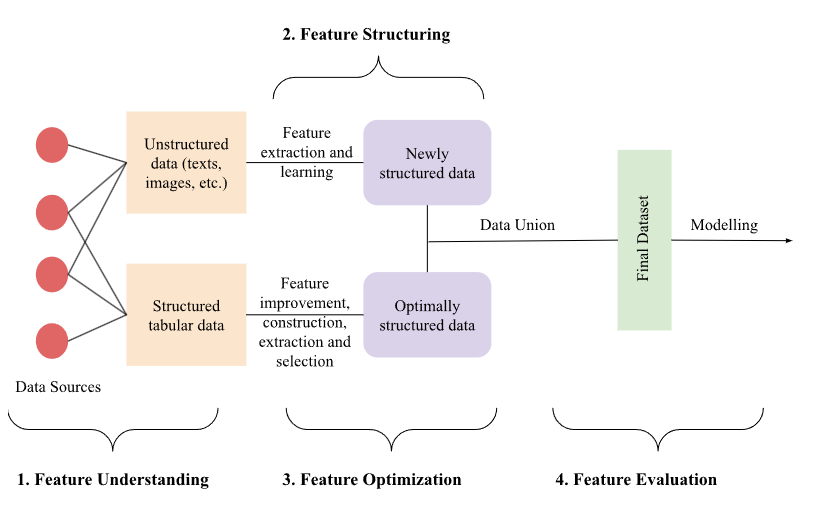
\includegraphics[width=\textwidth]{figures/datasets-and-features}
	\caption{Datasets and Features}
	\label{fig:datasets-and-features}
\end{figure}

\section{Feature Scaling}\label{sec:feature-scaling}
\emph{Scale} the data to a fixed range \data{$[0, 1]$}.
\begin{itemize}
	\item \definition{Normalization}{Rescale the \emph{data} \data{$x$} using the \emph{mean} \data{$(\mu)$} and the \emph{standard deviation} \data{$(\sigma)$} of the data.}
	\begin{equation}
		\data{x_{norm} = \frac{x - \mu}{\sigma}}
		\label{eq:normalization}
	\end{equation}
	\item \emph{Min-Max Scaling}:
	\begin{equation}
		\data{x_{minmax} = \frac{x - x_{min}}{x_{max} - x_{min}}}
		\label{eq:min-max-scaling}
	\end{equation}
\end{itemize}

\section{Types of Datasets}\label{sec:types-of-datasets}
\begin{itemize}
	\item Numerical Dataset.
	\item Categorical Dataset.
	\item Web Dataset.
	\item Time series Dataset.
	\item Image Dataset.
	\item Ordered Dataset.
	\item Bivariate Dataset.
	\item Multivariate Dataset.
\end{itemize}

\section{The Task, $T$}\label{sec:the-task}
Tasks are usually described in terms of how the machine learning should process an example: \data{$x\in\mathbb{R}^{n}$} where each entry \data{$x_{1}$} is a \emph{feature}.
\begin{description}[font=\color{emphblue}]
	\item[Classification:] Learn \data{$f: \mathbb{R}^{n}\rightarrow\{1,\dots,k\}$}
	\begin{itemize}
		\item \data{$y=f(x)$}: \emph{assigns input} to the \emph{category} with \emph{output} \data{$y$}.
		\item Example: Object recognition
	\end{itemize}
	\item[Regression:] Learn \data{$f: \mathbb{R}^{n}\rightarrow\mathbb{R}$}
	\begin{itemize}
		\item Example: Weather prediction, real estate price prediction.
	\end{itemize}
\end{description}

\end{document}